\documentclass[a4paper,12pt]{scrartcl}
\usepackage[francais]{babel}
\usepackage[utf8]{inputenc}
\usepackage[T1]{fontenc}
\usepackage[a4paper,margin=0.75in]{geometry}
\usepackage{pdflscape}
\usepackage{tabularx}
\usepackage{diagbox}
\usepackage{tikz}

\renewcommand{\arraystretch}{2.8}

\begin{document}

\title{Mesures Binaires}
\author{Marie Le Guilly \and Clément Mommessin}

\maketitle

%%%%%%%%%%%%%%%%%%%%%%%%%%%%%%%%%%%%%%%%%%%%%%%%%%%%%%%%%%%%%%%%%%%%%%%%%
\section{Notions abordées}

Le but de cette activité est de découvrir le langage binaire et de voir comment sont représentés ces nombres binaires dans un ordinateur.
La durée de l'activité peut varier de 30 minutes environ à 1h.


%%%%%%%%%%%%%%%%%%%%%%%%%%%%%%%%%%%%%%%%%%%%%%%%%%%%%%%%%%%%%%%%%%%%%%%%%
\section{Public}

Pour le moment l'activité a été testée seulement sur une classe de 3ème, mais il est possible de la faire pour toute classe de collège (voire fin de primaire pour la partie mesures et tri).

Pour une classe de lycée, la partie de tri peut être faite plus rapidement, laissant du temps pour aborder plus en details la manipulation des nombres binaires comme par exemple l'addition et la multiplication.



%%%%%%%%%%%%%%%%%%%%%%%%%%%%%%%%%%%%%%%%%%%%%%%%%%%%%%%%%%%%%%%%%%%%%%%%%
\section{Matériel}

Des réglettes en papier (ou tout autre morceau de bois, de carton) de taille 1, 2, 4, 8, 16, 32 (et ainsi de suite en doublant la taille de la réglette précédente), avec un symbole différent pour chaque longueur. Il est important de ne pas noter les tailles sur les réglettes, mais seulement des symboles !

L'appendice A propose une page à imprimer contenant 2 jeux de réglettes de taille allant de 1 à 32 (coller les parties en pointillés sous les trèfles pour la taille 32).\\


Au moins 6 objets à mesurer. Prévoir des objets au minimum de taille 1 et au maximum de taille 2 fois la plus grande réglette moins 1, pour être capable de les mesurer.

Ces objets peuvent cacher une lettre, ou directement être des lettres, pour voir se former un mot ou une phrase lorsqu'ils sont rangés du plus petit au plus grand.
Une liste d'ojets peut contenir par exemple les lettres pour former le mot "ordinateur" avec les tailles 5, 17, 23, 28, 37, 44, 46, 53, 56 et 60.\\
Lors de l'activité, les lettres du premier groupe étaient O (5), D (23), N (37), E (53) et R (60). Pour le second groupe R (17), I (28), A (44), T (46) et U (56).
\textcolor{red}{A vérifier avec Pascal qui a gardé les cartons. A voir si une autre répartition des lettres serait mieux.}\\

L'appendice B présente deux tableaux qui peuvent être distribués aux groupes pour aider à noter la taille des objets en termes de symboles.



%%%%%%%%%%%%%%%%%%%%%%%%%%%%%%%%%%%%%%%%%%%%%%%%%%%%%%%%%%%%%%%%%%%%%%%%%
\section{Principe}

L'activité se fait principalement en deux groupes séparés, chacun disposant de la moitié des objets.
Le but est d'ordonner l'ensemble des objets des deux groupes du plus grand au plus petit, en utilisant les réglettes mises à disposition.

Chaque objet se mesure en utilisant une ou plusieurs réglettes, et il n'est pas possible de faire des "soustractions de réglettes" (par exemple "cet objet mesure une réglette trèfle moins une réglette carreau").\\


Une fois que chaque groupe a mesuré ses propres objets, l'échange de mesures entre les deux groupes pour ordonner l'ensemble des objets ne doit se faire qu'en termes de symboles.

Penser à noter sur un grand tableau récapitulatif l'ensemble des objets triés et leur composition en terme de symboles (en écrivant le symbole correspondant à la plus grande réglette à gauche, puis décroissant vers la droite) pour faire apparaître la notation binaire. Le tableau d'une salle de classe est très pratique pour ça !\\


Une étude des réglettes permet de voir qu'en partant de la plus petite réglette, que l'on associe à la taille unitaire 1, chaque réglette plus grande est le double de la réglette d'avant. 
%
Chaque réglette a une taille qui est une puissance de 2, on peut donc associer chaque symbole à cette taille. Ainsi, il est possible d'écrire la taille de chaque objet non pas en terme de symbole mais de nombre (un certain nombre de fois la taille unitaire), ce qui facilite l'opération de tri des objets.

On introduit ainsi l'écriture binaire des nombres.
On peut ajouter que la représentation binaire est unique, et que l'on peut mesurer tous les objets entre 1 et 63 si la plus grande réglette est 32 (en écartant les tailles qui ne sont pas "entières") et donc écrire tous les nombres entre 0 et 63.


%%%%%%%%%%%%%%%%%%%%%%%%%%%%%%%%%%%%%%%%%%%%%%%%%%%%%%%%%%%%%%%%%%%%%%%%%
\section{Extensions}

Pour aller plus loin, on peut parler de l'addition et de la multiplication de deux nombres binaires (la soustraction est plus compliquée !).

On peut aussi aborder la notion d'algorithme de mesure : comment choisir efficacement les réglettes pour mesurer un objet ? On peut aller d'un algo naïf (on essaie toujours la plus grande réglette et on descend), à plus avancé (recherche dichotomique de la réglette la plus proche en taille mais plus petite que l'objet).

Enfin, on peut conclure sur un petit tour de magie permettant au "magicien" de deviner un nombre pensé par le public en passant d'un nombre représenté en binaire vers sa notation décimale.
\textcolor{red}{Ajouter tableaux ou URL d'une page web qui l'explique déjà.}



%%%%%%%%%%%%%%%%%%%%%%%%%%%%%%%%%%%%%%%%%%%%%%%%%%%%%%%%%%%%%%%%%%%%%%%%%
\section{Photos}

\begin{figure}
\begin{center}
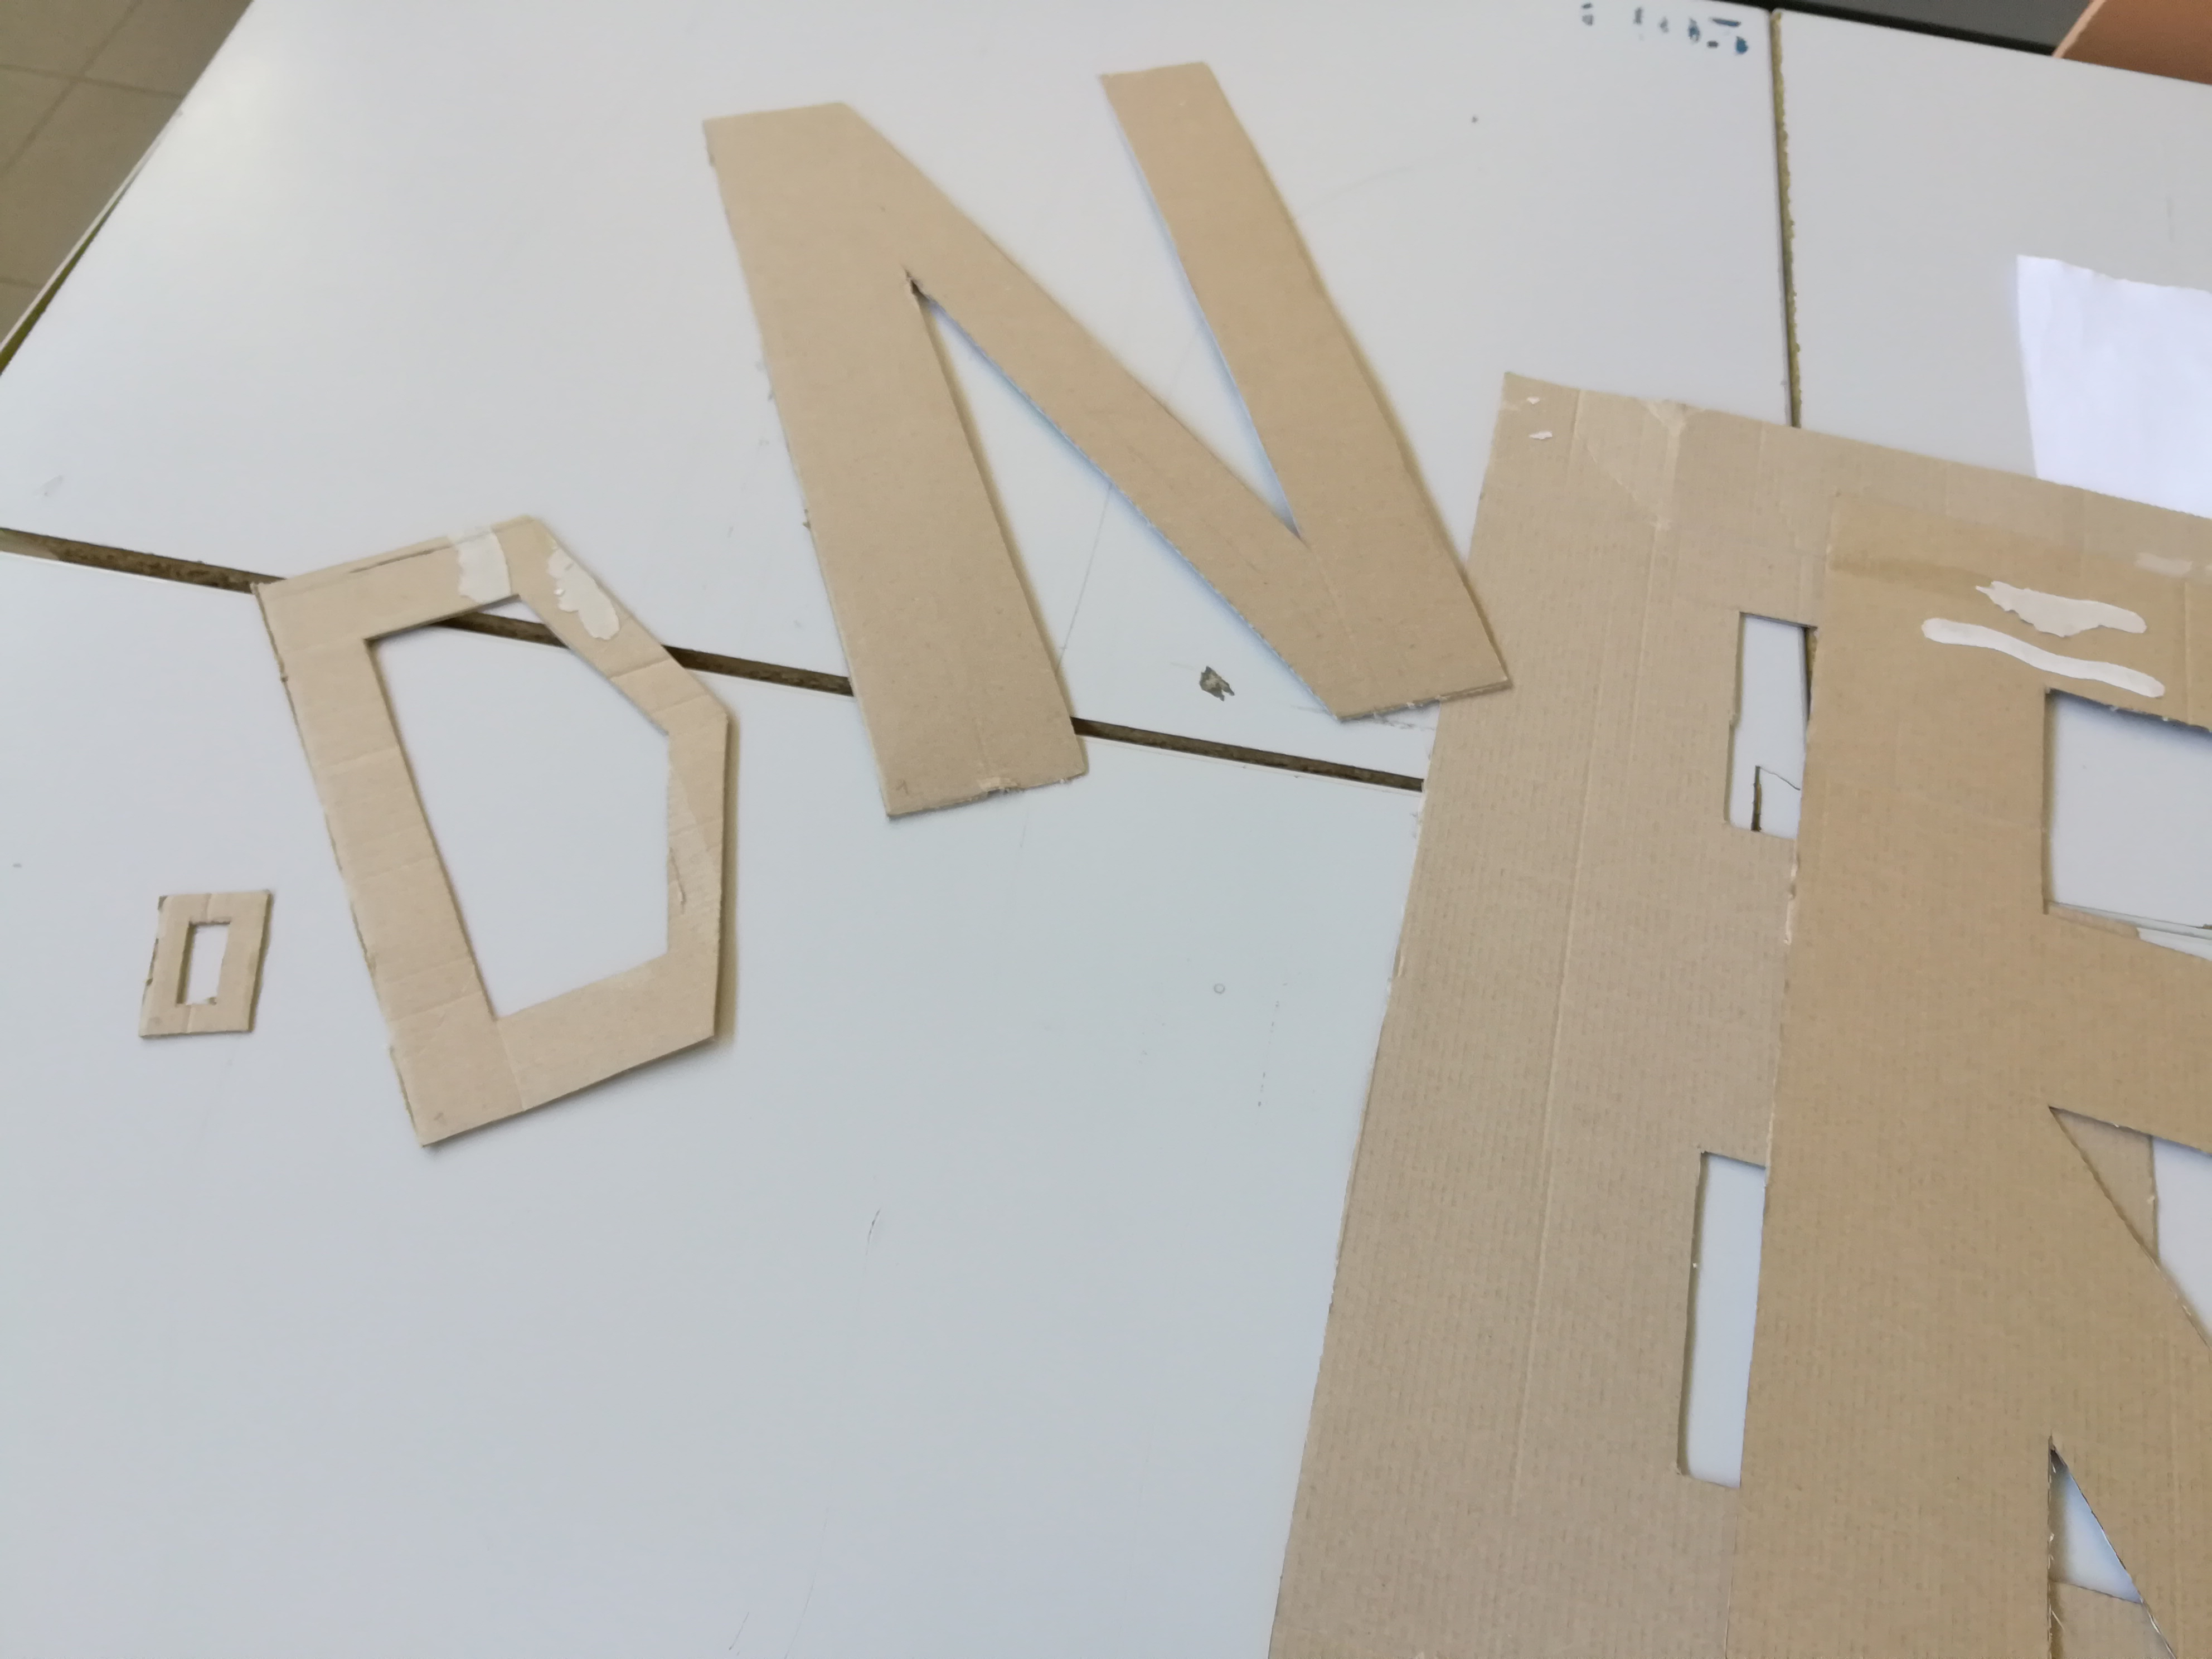
\includegraphics[width=0.7\linewidth]{images/lettres.jpg} 
\end{center}
\caption{Exemples de lettres découpées dans du carton}
\label{fig:lettres}
\end{figure}

\begin{figure}
\begin{center}
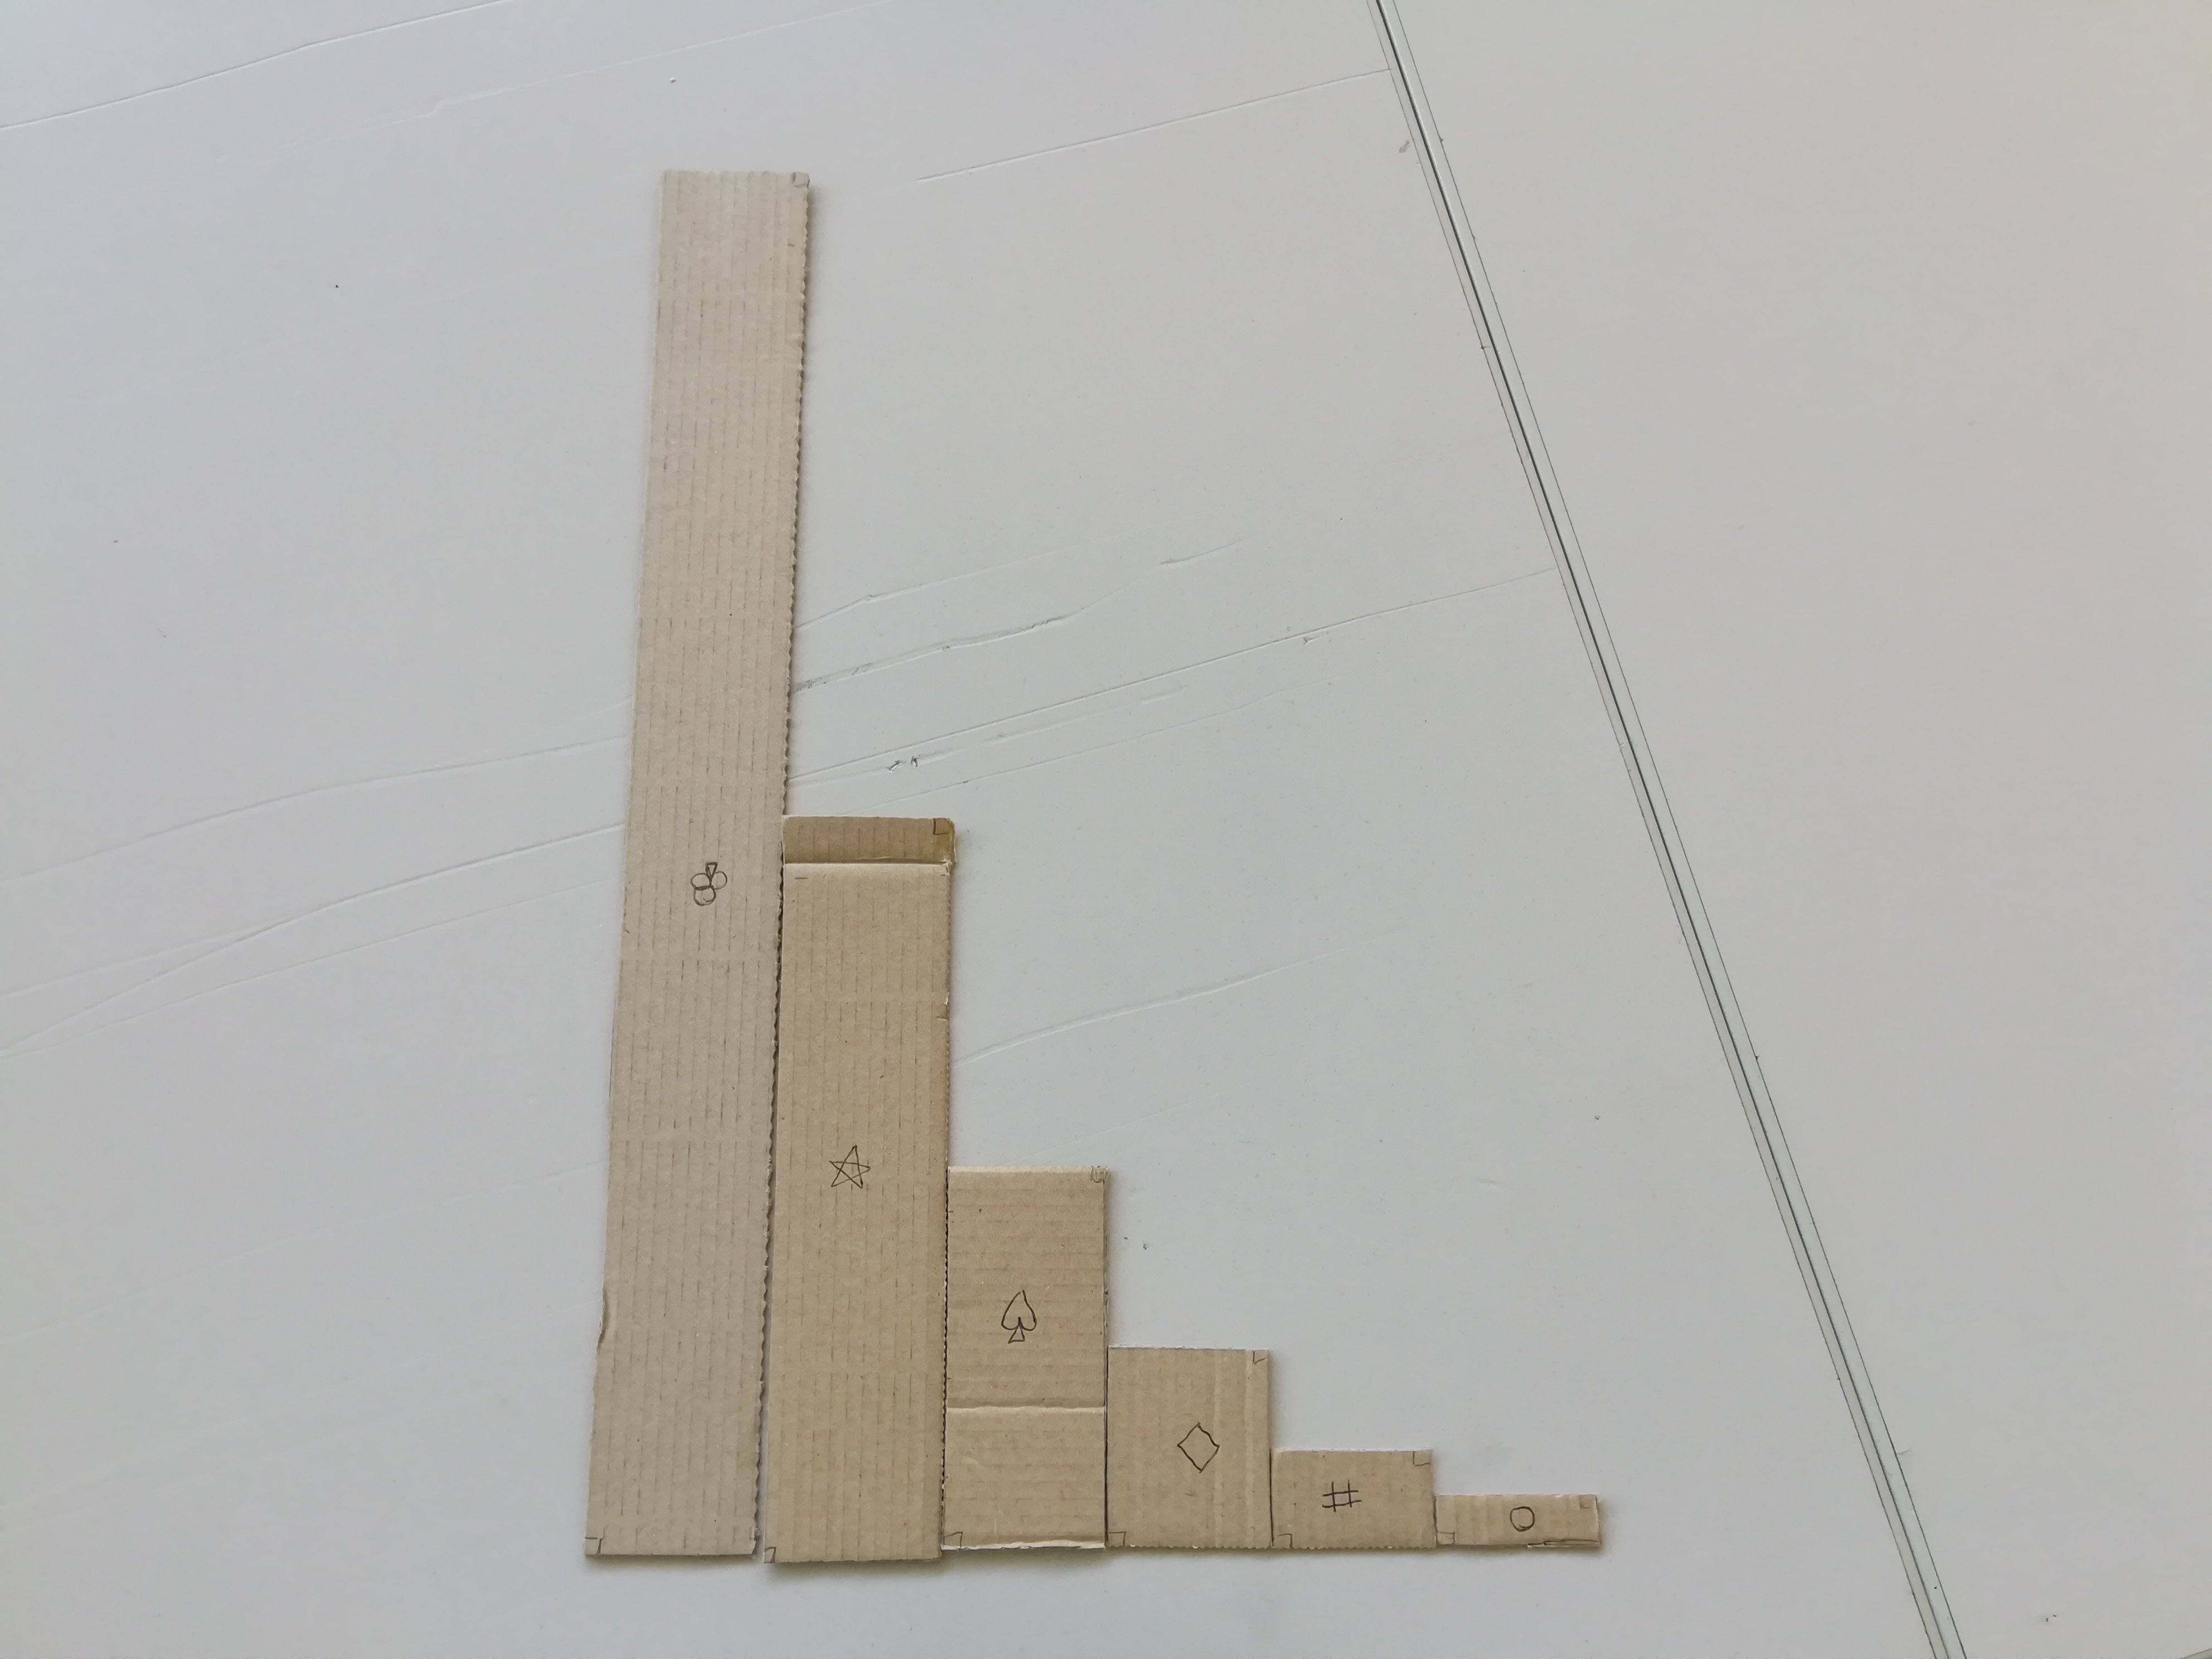
\includegraphics[width=0.7\linewidth]{images/reglettes.jpg} 
\end{center}
\caption{Exemples de réglettes en carton}
\label{fig:lettres}
\end{figure}

\begin{figure}
\begin{center}
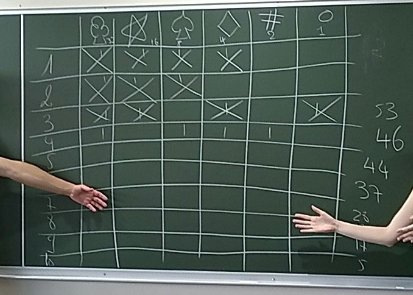
\includegraphics[width=0.7\linewidth]{images/tableau.png}
\end{center}
\caption{Conclusion de l'activité au tableau, des symboles aux nombres binaires}
\label{fig:lettres}
\end{figure}

\newpage
~\\
\newpage
\appendix
%%%%%%%%%%%%%%%%%%%%%%%% RECTANGLES %%%%%%%%%%%%%%%%%%%%%%%%%
\thispagestyle{empty}
\bf{Appendice A :} 2 jeux de réglettes de taille 1, 2, 4, 8, 16 et 32.
\bigskip
\bigskip
~\\

\begin{tikzpicture}
    \draw (0,0) rectangle (4,3);
    \draw (4,0) rectangle (8,3);
    \draw (8,0) rectangle (10,3);
    \draw (10,0) rectangle (12,3);
    \draw (0,3) rectangle (8,6);
    \draw (8,3)rectangle (16,6);
    \draw (0,6) rectangle (16,9);
    \draw (16,6) rectangle (17,9);
    \draw (0,9) rectangle (16, 12);
    \draw (16,9) rectangle (17,12);
    \draw (0,12) rectangle (17,15);
    \draw (0,15) rectangle (17,18);
    \draw (0,18) rectangle (17,21);
    \draw (0,21) rectangle (17,24);
    \draw[dashed] (15,12) -- (15,18);

    \draw (16.5,7.5) node[scale=1.75]{$\circ$};
    \draw (16.5,10.5) node[scale=1.75]{$\circ$};
    \draw (16,19.5) node{$\clubsuit$};
    \draw (16,22.5) node{$\clubsuit$};
    \draw (8,10.5) node[scale=1.75]{$\star$};
    \draw (8,7.5) node[scale=1.75]{$\star$};
    \draw (4, 4.5) node{$\spadesuit$};
    \draw (12, 4.5) node{$\spadesuit$};
    \draw (2, 1.5) node{$\diamondsuit$};
    \draw (6, 1.5) node{$\diamondsuit$};
    \draw (9, 1.5) node{$\#$};
    \draw (11, 1.5) node{$\#$};
\end{tikzpicture}

\newpage
\thispagestyle{empty}
\bf{Appendice B :} 2 tableaux d'aide pour la représentation des mesures
\bigskip
\bigskip
~\\

\begin{tabularx}{\hsize}{|c|X|X|X|X|X|X|}
    \hline
    \diagbox{Objet}{Composition} & & & & & & \\
    \hline
     & & & & & & \\
    \hline
     & & & & & & \\
    \hline
     & & & & & & \\
    \hline
     & & & & & & \\
    \hline
     & & & & & & \\
    \hline
\end{tabularx}

\vspace{.5in}


\begin{tabularx}{\hsize}{|c|X|X|X|X|X|X|}
    \hline
    \diagbox{Objet}{Composition} & & & & & & \\
    \hline
     & & & & & & \\
    \hline
     & & & & & & \\
    \hline
     & & & & & & \\
    \hline
     & & & & & & \\
    \hline
     & & & & & & \\
    \hline
\end{tabularx}

\end{document}